\section{Relative Position and Velocity Estimation}

%\subsection{System Architecture}
%\begin{frame}{\thesection. \insertsection \ - \insertsubsection}
\begin{frame}{MAV Sensor Suite}
	%\begin{figure}
		\begin{center}
		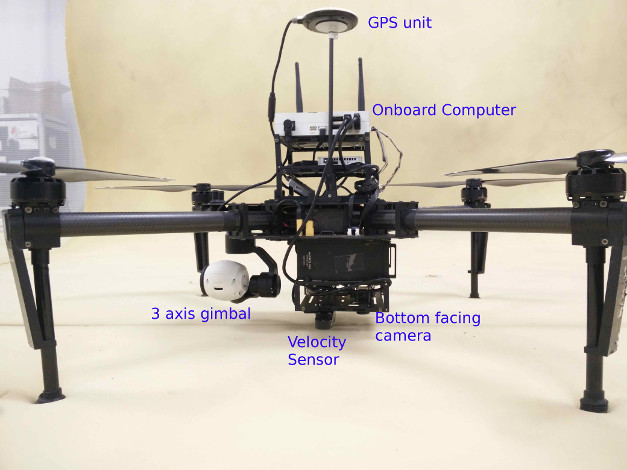
\includegraphics[width=0.5\paperwidth]{figures/m100.jpg}
		\end{center}
		%\caption{
		\vspace{-0.5cm}
		DJI M100 equipped with: 
		\begin{itemize}
			\item Onboard integrated navigation system (INS) fusing data from GPS, IMU and velocity sensor (optical flow)
			\item 3-axis gimbal and a bottom facing wide angle camera for AprilTag detection
		\end{itemize}
		%}
	%\end{figure}
\end{frame}

% ----------------------------------------------------------------------

%\begin{frame}{\thesection. \insertsection \ - \insertsubsection}
\begin{frame}{GV and Landing Platform}
	\begin{figure}
		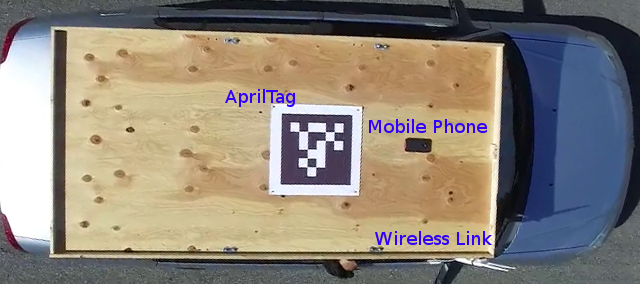
\includegraphics[width=0.8\paperwidth]{figures/car.png}
		%\caption{
		\begin{itemize}
			\item	AprilTags allow for robust 6DoF visual pose estimation in real-time %by solving a least squares problem after extracting the 4 corners of the tag 
			\item Mobile phone provides IMU and GPS data (slow, low accuracy), transmitted to MAV via long-range WiFi link
		\end{itemize}
	%}
	\end{figure}
\end{frame}

% ----------------------------------------------------------------------

%\subsection{Kalman Filter}
%\begin{frame}{\thesection. \insertsection \ - \insertsubsection}
\begin{frame}{Kalman Filter}
	%\begin{figure}
		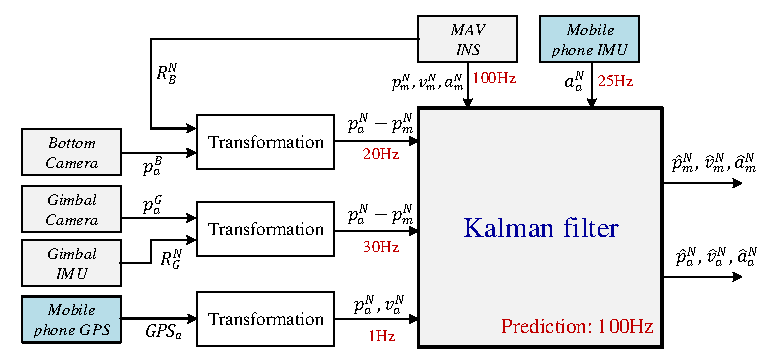
\includegraphics[width=0.85\paperwidth]{figures/kf.pdf}\\
		%\caption{Estimator inputs and outputs. 
		\begin{itemize}
			\item $m$: MAV, $a$: AprilTag (or GV). $N$: navigation frame.
			\item	MAV attitude est. $R^N_B$, gravity compensated $a_m^N$ from INS\ldots %takes care of the MAV's non-linearities for us.
		\end{itemize}
		%}
	%\end{figure}
\end{frame}

% ----------------------------------------------------------------------

%\subsection{Kalman Filter}
%\begin{frame}{\thesection. \insertsection \ - \insertsubsection}
%	Process model
%\end{frame}

% ----------------------------------------------------------------------

%\subsection{Kalman Filter}
%\begin{frame}{\thesection. \insertsection \ - \insertsubsection}
%	Measurement model
%\end{frame}

% ----------------------------------------------------------------------